\documentclass[11pt]{article}
\usepackage[top=1in, bottom=1in, left=1in, right=1in]{geometry}
\usepackage{float}
\usepackage{color}
\usepackage{picture}
\usepackage{listings}
\usepackage{caption}
\usepackage{makeidx}
\usepackage{graphicx}
\usepackage{amsmath}
\usepackage{subcaption}
\usepackage[utf8]{inputenc}
\usepackage[linktocpage=true]{hyperref}

% Used for the figures that have been inserted into the document.
\floatstyle{plain} 
\restylefloat{figure}

% Used so as not to indent paragraphs.
\setlength\parindent{0pt}

% Used for syntax highlighting in code.
\definecolor{skyblue}{rgb}{0.53, 0.81, 0.92}
\definecolor{lightred}{rgb}{0.90, 0.36, 0.36}
\definecolor{darkkhaki}{rgb}{0.71, 0.51, 0.06}

% Default parameters for listings package.
\lstset {
	tabsize=4,
	keywordstyle=\color{darkkhaki},
	commentstyle=\color{blue},
	showstringspaces=false,
	stringstyle=\color{lightred},
	frame=TLRB,
	captionpos=b,
	basicstyle=\small\ttfamily,
	breaklines=true
}

% Default parameters for hyperref package.
\hypersetup {
	pdftoolbar=true,
	pdfmenubar=true,
	colorlinks=true,
	linkcolor=red,
	citecolor=green,
	filecolor=magenta,
	urlcolor=cyan
}

\newcommand{\superscript}[1]{\ensuremath{^{\textrm{#1}}}}
\newcommand{\subscript}[1]{\ensuremath{_{\textrm{#1}}}}

\numberwithin{equation}{section}
%\setcounter{secnumdepth}{0}
\begin{document}

\begin{titlepage}

\begin{center}

\textsc{\LARGE Risk Management}\\[2.5cm]

\linethickness{0.5mm}
\line(1, 0){1\linewidth} \\[0.4cm]
{\huge \bfseries Value at risk, Credit risk} \\[0.4cm]
{\huge \bfseries and Credit derivatives}
\line(1, 0){1\linewidth} \\[2.5cm]

\begin{minipage}[t]{0.4\textwidth}
	\begin{flushleft} \large
	\emph{Prepared by:} \\[0.3cm]
	Nikhil Agarwal \\
	{\small 11012323} \\[0.2cm]
	Vishal Keshav \\
	{\small 11012341} \\[0.2cm]
	\end{flushleft}
\end{minipage}
\begin{minipage}[t]{0.4\textwidth}
	\begin{flushright} \large
	\emph{Supervisor:} \\[0.3cm]
	Dr. Siddhartha P. Chakrabarty 
	\end{flushright}
\end{minipage}

\vfill

% Bottom of the page
{\large \today}

\end{center}

\end{titlepage}

\pagebreak

\renewcommand\contentsname{{\Huge Contents}\vspace{0.5cm}}
\addtocontents{toc}{~\hfill\textbf{Page}\par}
\cleardoublepage
\phantomsection
\addtocontents{toc}{\linespread{1.5}\selectfont}
\addcontentsline{toc}{section}{Contents}
\setcounter{tocdepth}{8}

\tableofcontents

\cleardoublepage
\phantomsection
%\addcontentsline{toc}{section}{List of Figures}
\renewcommand\listfigurename{{\Huge List of Figures}\vspace{0.5cm}}
\addtocontents{lof}{\linespread{1.5}\selectfont}
\addtocontents{lof}{~\hfill\textbf{Page}\par}
%\listoffigures

\pagebreak

\section{Value at risk}
\medskip
\subsection{Introduction}
\medskip
Now a days risk management is the primary requirement of all the investment . There are several risk measures such as delta, gamma, etc . They are useful only when portfolio consist of derivatives dependent on single market variables but what happens when our portfolio consist of several market variables ? In that case we need a unified number to represent risk the company holds on it's portfolio. Thus, Value at Risk (VaR) is an attempt to provide a single number summarizing the total risk in a portfolio of financial assets .  
\medskip
\subsection{Estimating VaR}
\medskip
While estimating VaR we don't give the exact number but we say that it will not exceed some specified number with certain probability in the given time horizon. This probability is called \textbf{Confidence level}. VaR is actually a function of confidence level and number of days. In general, when N days is the time horizon and X\% is the confidence level, VaR is the loss corresponding to $ (100-X) $th percentile of the distribution of the change in the value of portfolio over the next N days. We assume in most of the cases the change in return follows normal distribution. \medskip

\begin{figure}[H]
		\centering
		\resizebox{0.6\linewidth}{!}{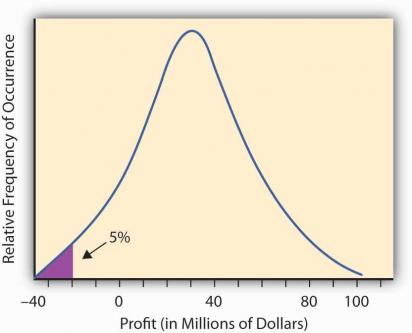
\includegraphics{fig1}}
		\caption{Normal distribution with confidence interval 95\%}
		\label{fig:q1_f1_a}
\end{figure} 

\subsection{Calculation of VaR}
There are basically two ways to calcualte VaR. They are \textbf{HISTORICAL SIMULATION} and \textbf{MODEL BUILDING APPROACH}.
\pagebreak

	\subsubsection{Historical Simulation}
	\medskip
 In this model we take some recent 500 or 1000 days of data to estimate the values of VaR. From those data we simulate 500 or 1000 scenarios for next day portfolio's value and assume each scenario have equal probability of occurrence.\medskip
	
	\hspace{1cm} Assume  $v_i$ as the value of a market variable on day i and if today is day m, then the ith scenario will have the value $v_m$ $\frac{v_i}{v_{i-1}}$. If we have 90\% confidence level and 1000 scenarios the we chose 100th worst case scenario as our percentile point which represents our VaR. 
	\subsubsection{Model Building Approach}
	\medskip
	\begin{enumerate}
		\item\textbf{Linear Model}
		\medskip
				
		If our portfolio consist of assets and derivatives depending on some n market variables then the change in portfolio is equal to a linear combination of change in these n market variables which is given by
\begin{center}
 $ {\Delta}P  =  \sum_{i=1}^n{\alpha_i}{\Delta}{x_i} $
\end{center}
	where ${\Delta}P $ is the change in the value of portfolio,
	$\alpha_i$ is the amount invested in asset i and ${\Delta}{x_i}$  is return on asset i.
		  In general case we assume that the market variable follows multivariate normal distribution. Thus the change in value of portfolio follows normal distribution. Determining the volatility of change in value of portfolio, we can determine percentile point given some confidence interval. This percentile point is representation of VaR. 
		
		\begin{enumerate}
		\item\textbf{Single Asset Case}
		\medskip
		
		In this case we have a portfolio dependent on single market variable. If this market variable follows normal distribution then change in the value of portfolio follows normal distribution. For example, if we have a portfolio of Rs.100000 worth shares in a company A and if the volatility is 1\% standard deviation of change in portfolio will be $ 100000*0.01=1000 $ . Then 99\% VaR is $ 2.33*1000=2330 $.
		\medskip
		
		 \item\textbf{Two Asset Case} 
		 \medskip
		 
		In this case we assume there are two companies A and B with standard deviation $ \sigma_A $ and $ \sigma_B $ and coefficient of correlation between them is $\rho $ . If our portfolio consist of assets of both companies then the standard deviation of the change in value of the portfolio will be given by $ \sigma $ =  $\sqrt{\sigma_A^{2}+\sigma_B^{2}+2\rho\sigma_A\sigma_B}$ . The value of 1 day 99\% var is  $2.33\sigma$. 
		\end{enumerate}
	\textbf{Applications}\medskip
	\begin{itemize}
	\item It can be used in portfolio with no derivatives consisting of positions in stocks, bonds, etc.
	\item In case of portfolio consisting of bonds cash-flow mapping can be used.  
	\item If a portfolio consist of derivative then derivative can be converted to zero coupon bonds hence cash flow mapping is utilized.
	\item If a portfolio consist of options then only delta of  the option is taken into account under this model . If the stock price is S then the change in value of portfolio is given by $\Delta P$ = $\delta \Delta S $.
	\end{itemize}
	\pagebreak
	
	\item\textbf{Quadratic Model}\medskip
	
	If our portfolio include options then linear model is an approximation. It does not take into account the rate of change of delta with respect to market variable which is gamma of the portfolio. Then, the equation becomes \medskip
	\begin{center}
	$\Delta P$ = $\delta \Delta S + \frac{1}{2}\gamma (\Delta S)^{2}$
	\end{center}
	setting $\Delta x$ = $\frac{\Delta S}{S}$ the euation reduces to
		\begin{center}
	$\Delta P$ = $S\delta \Delta x + \frac{1}{2} S^{2}\gamma (\Delta x)^{2}$
	\end{center}
	If portfolio consist of n options then the change in portfolio for all asset becomes
	\begin{center}
	$\Delta P$ = $\sum_{i=1}^n S_i\delta_i \Delta x_i + \sum_{i=1}^n \frac{1}{2} S_i^{2}\gamma_i (\Delta x_i)^{2}$
	\end{center}
	where i denotes ith asset. 
	\item\textbf{Monte Carlo Simulation}\medskip
	
	We use Monte Carlo simulation to generate probability distribution for $\Delta P $ . The steps are as follows: 
	\begin{enumerate}
	\item Sample once from multivariate normal probability distribution of $ \Delta x_i $ .
	\item $ \Delta x_i $ sampled in step(a) are change in the value of market variable.
	\item Value of portfolio is determined using the above data.
	\item We determine the sample $\Delta P$ by subtracting the value of portfolio today from value in step(c).
	\item Repeat the step (a) to (d) to build probability distribution of $\Delta P$.
	\end{enumerate}
	\end{enumerate}
	

\subsection{Stress Testing and Back Testing}\medskip

\textbf{Stress Testing} involves estimating how the portfolio would have performed under some of the most extreme market moves seen in last 10 to 20 years. Thus, by looking over extreme scenarios of past 10 to 20 years we estimate the condition of our survival if such a scenario happens next day.  \textbf{Back Testing} involves looking at how often the loss in a day exceeded the 1 day 99\% VaR that would have been calculated for that day. Thus we estimate the frequency of our loss using the past data.

\subsection{Principal Component Analysis}

This approach is used to handle risk by taking historical data on movements in market variables and defining factors that explains the movement. Here we have varying change in rate for each of the maturities of a particular factor. Each Factor have different significance and can correspond to parallel shift or steepening or bowing of the yield curve. The interest rate move for a particular factor is called \textbf{factor loading}. The quantity of a particular factor in the interest rate changes on a particular day is known as factor score for that day. The importance of a factor is measured by standard deviation of its factor score. By adding these variances of factor scores we get total variance of the data. By dividing variance of each factor by total variance we get the percentage contribution of each factor in the risk of portfolio.

\subsubsection{Calculation Of VaR Using Principal Component Analysis}
\medskip

As the first two-three factors having large variances contribute mostly to the risk and rest are quite smaller we can calculate our exposures for these two-three factors. This can be done by multiplying interest rate for a given maturity by the change in portfolio value. After that we multiply each of these exposures to their factor scores and find the total change in portfolio by adding them. Then, we can easily calculate the standard deviation of change in portfolio. For calculating 1-day X\% var we can multiply the standard deviation with the corresponding value to get VaR. Thus, for a VaR calculation it would be most appropriate to carry out a principal components analysis on percentage change in market variable rather than actual changes.  

\pagebreak
\section{Credit risk}
\medskip

\subsection{Introduction}
\medskip

Credit risk refers to the risk that a borrower will default on any type of debt by failing to make payments which it is obligated to do. Credit risk arises when a consumer may fail to make a payment due on a mortgage loan, credit card or a company is unable to repay amounts secured by a fixed or floating rate  over the assets of the company

\subsection{Credit Ratings}
\medskip

There are several rating agencies such as Moody's and S\&P. They provide credit worthiness rating to corporate bonds. For example, S\&P gives AAA rating to \textbf{investment grade} bonds. Different kinds of rating are AAA, AA, A, BBB, BB, B, CCC. AAA rating bonds are least probable to default while CCC rating bonds are most probable to default. Probability of default for investment grade bonds in a year increases with respect to time. The possibility of declination of potential health of a company issuing the bond increases as time elapses. Probability of default in a year for poor credit rating bonds decreases with time. The reason for this is if the issuer survives this period it's financial health is likely to have improved. 

\subsection{Estimating Default probabilities}
\medskip

\subsubsection{Estimation from Historical data}
\medskip

Rating agency produces historical data which shows
the default experience through time of companies that started with certain credit rating. 
\begin{itemize}
\item\textbf{Default Intensities}
\medskip

Default Intensities are conditional default probability in a given year provided that the company has not been defaulted prior to that year. The cumulative probability of the company surviving to time t is given by 
\begin{center}
	\textbf{$ V(t) $ = $ e ^{-\int_0^{t} \lambda (t)\,d \tau }$}
\end{center}
where $\lambda (t)$ is default intensity. The probability of default by time t is give by $Q(t)$ = $1-V(t)$

\item\textbf{Recovery Rate}
\medskip

Amount recovered through bankruptcy processors in event of default expressed as percentage of face value is called recovery rate. If the recovery rate is R\% then at the time of default the amount recovered is given by $ principal*R $. \textbf{Recovery rates are negatively correlated with default rates}.

\end{itemize}

\subsubsection{Estimation from bond price}
\medskip

 If a company sells a corporate bond priced less than similar risk free bond then there is a chance of default. 
Given recovery rate R the estimation of probability of default per year conditional on no earlier default is h given by 
\begin{center}
	$ h $ = $\frac{s}{1-R}$
\end{center}
where s is spread of corporate bond yield over the risk free rate.
\begin{itemize}
\item \textbf{Calculation}
\medskip

First of all, we determine the price of corporate bond and risk free bond from given yield. Then, the expected loss from default over the life of bond is given by difference of risk free bond and corporate bond. Let the difference be d.\medskip

 \hspace{1cm}We now assume Q to be default probability per year which is assumed to be same over the life of bond. We then calculate loss from default on the corporate bond by calculating present value of the expected loss in terms of Q over the lifetime of the bond. Adding all the calculated losses, we get the total expected loss. When, we equate this value with d, we get the value of default probability per year.
 
 \item \textbf{Asset Swap}
 \medskip
 
 Through asset swaps, there are exchanges of coupon on a bond for LIBOR + spread. Asset swap spread are used to extract default probabilities from bond prices. The present value of asset swap spread is the amount by which the price of corporate bond is exceeded by the price of similar risk free bond. The amount by which the value of risk free bond exceeds the value of corporate bond is present value of the basis points per year.
 for example, suppose the two companies quotes an asset swap spread for a particular bond at x basis points. If selling  value of a bond is same as it's par value then company A will pay the coupons while the company B will pay LIBOR + x basis points. If selling value is lower then company A will pay the difference and coupons and if the selling value is higher company B will pay LIBOR + spread + the difference. 
   
\end{itemize}

\subsubsection{Comparison of Default Probability Estimates }
\medskip

First of all we tabulate the historical default intensities and default intensities from bonds for different ratings. Then we calculate the ratio and difference of default intensity from bonds and historical data for different ratings. It is observed that as risk increases, the ratio declines and difference increases.

\subsubsection{Real World vs. Risk Neutral probabilities}
\medskip

The default probability we calculated using historical data is real world probability while probabilities from bond prices are risk neutral probabilities. The reason for this is that the calculation assumes that expected default loss can be discounted at risk free rate which we made during estimation of default probabilities from bond prices. When valuing credit derivatives or estimating the impact of default risk on the pricing of the instruments we should use risk neutral probability. When carrying out scenario analysis to calculate potential future losses from default we use real world default probabilities.

\subsubsection{Estimation using equity prices}
\medskip

Equity is the value of an asset after all the liabilities and debts have been paid. We use the Merton model and consider companies equity as an option on the assets of the company. It is considered as an option because if value of company's asset at time T ($ V_T $) is less than amount of debt ($ D $) due to be repaid at time T then company defaults and the value of equity is 0 but if $V_T$ is greater than $ D $ then company will repay the debt and equity becomes $V_T-D$. From, Black-Scholes formula value of equity today is given by 
\begin{center}
	$ E_0 = V_0 N(d_1) - De^{-rT} N(d_2)$
\end{center}  
where
\begin{center}
	$ d_1= \frac{ln {V_0}/{D} + (r+\sigma_V^{2}/2)T}{\sigma_V \sqrt{T}} $ and $ d_2 = d_1 - \sigma_V \sqrt{T}$
\end{center}
where $V_t$ is company's asset at time t, $E_t$ is the company's equity at time t, $\sigma_V $ is volatility of assets.\medskip

\hspace{1 cm} Value of debt today is $V_0 - E_0 $. \textbf{Risk Neutral probability that the company will default is $N(-d_2)$ }. From It\^{o}'s lemma we determine unknown $V_0$ and $\sigma_V$ by using
\begin{center}
	$ \sigma_E E_0 $ = $ N(d_1)\sigma_V V_0 $
\end{center}  

\subsection{Credit risk in derivative transactions}
\medskip

Consider that financial institution has a derivative with counterparty. Then, we have three possible situations:
\begin{itemize}
\item Case 1: In this case, Contract is always an asset to financial institution. Here, financial institution has credit risk because if party goes bankrupt, it will cause loss to financial institution. Considering R as recovery rate and $ q_i$ as probability of default at time  $ t_i $. Then total risk neutral expected loss from default is $\sum_{i=1}^n u_i v_i $ where $u_i $ is $q_i(1-R)$ and $ v_i $ is today's value of an instrument that pays off the exposure on the derivative under consideration at time $t_i$
\item Case 2: In this case, contract is always a liability to financial institution. Here, financial institution has no credit risk because if party goes bankrupt, it will not cause any loss to financial institution. here, total risk neutral expected loss from default is zero.
\item Case 3: In this case, contract can become either an asset or liability to a financial institution. In this case, $max(f_i,0)$ is not predetermined. Then, we consider $v_i$ as a call option on $f_i$ with strike price zero. We simulate $v_i$ to calculate the risk neutral expected loss.
\end{itemize}

\subsection{Credit Risk Mitigation}
\subsubsection{Netting} 
\medskip

Netting is a clause which states that if a company defaults on one contract it has with a counterparty then it must default on all outstanding contracts with the counterparty. For example, suppose a financial institution A has three contacts with it's counterparty B of worth \$10, \$20, -\$30. Then, the contacts will worth  -\$10, -\$20, +\$30 to B. If B defaults on first contact then without netting he can gain \$10 but with netting he is compelled to default on all three contracts and will have no profit in the given scenario.\medskip

  \hspace{1cm} If a financial institution have a portfolio of N derivative contracts with a counterparty. Then, without netting financial institution losses $(1-R)\sum_{i=1}^N max(V_i,0) $ but with netting it losses $(1-R) max(\sum_{i=1}^N V_i,0)$ where R is recovery rate and $V_i$ is no default value of ith contract.
  
  \subsubsection{Collateralization}
  \medskip

   A collateralization agreement specifies that contract should be marked to market periodically using a pre-agreed formula. When the value of contact to financial institution is above a threshold level then it asks the company to post collateral. In the event of default by company, the financial institution can seize the collateral. For example, suppose the threshold value is \$10 million and marking is done on daily basis. If the value is more than \$10 million the institution will ask the company to pay the difference while on the other hand if it is less the company might ask to pay the collateral.
   
   \subsubsection{Downgrade Trigger}
   \medskip
   
   It is a clause stating that whenever the credit rating of a company fall below certain level then the financial institution has the option to close the derivative contract at it's market value. However, it do not provide protection in case of big jumps.     
   
   \subsection{Default Correlation}
   \medskip
   
Default correlation is used to describe the tendency for two companies to default simultaneously. Due to presence of default correlation, credit risk cannot be completely diversified away and this is the main reason why
risk-neutral probabilities are greater than real world default
probabilities.There are two types of model describing default correlation.
\begin{itemize}
\item \textbf{Reduced form models}: Under this model, it is assumed that default intensities for different companies follow stochastic processes and are correlated with macroeconomic variables. It reflects the tendencies of two companies to default around same point
of time. One disadvantage of this model is that, even when there is a perfect correlation between two default intensities, the corresponding correlation between defaults is usually too low.

\item \textbf{Structural models}: This model solves the difficulty faced in reduced form model. Default correlation between two companies are determined by assuming the stochastic process followed by the assets of the two company. 
are correlated.
\end{itemize}
\subsection{The Gaussian Copula Model for Time to Default}
\medskip

Under this model, it is assumed that company will ultimately default at some point of time. If we consider two companies defaulting at time point $t_1$ and $t_2$, the probability distribution of a company's time to default cannot be always considered normal. Thus $t_1$ and $ t_2 $ are transformed to $x_1$ and $x_2$ using $x_1$ = $N^{-1}[Q_1(t_1)]$ and $x_2$ = $N^{-1}[Q_2(t_2)]$ where $Q_1$ and $Q_2$ are the cumulative probability distribution for $t_1$ and $t_2$. This transformation is percentile to percentile transformation and this model of is called Gaussian Copula Model. $x_1$ and $x_2$  follow normal distribution with mean zero and unit standard deviation. We assume that the joint distribution of $x_1$ and $x_2$ is bivariate normal with correlation $\rho_{12} $. This assumption is referred to as using a Gaussian Copula. Similar arguments can be extended to n companies. 

\subsection{Using Factors to Define Correlation Structure}
\medskip

To avoid defining a different correlation between $x_i$ and $x_j$ for each pair of companies i and j in the Gaussian Copula model, \textbf{One-factor model} is often used. The assumption is $x_i$ = $a_iM + \sqrt{1-a^2}Z_i$. where M is common factor affecting defaults for all companies and $Z_i$ is a factor only affecting company i. The variables M and $Z_i$ are independent standard normal distributions. $a_i$ is constant factor between 1 and -1. The correlation between $x_i$ and $x_j$ is $a_ia_j$. Under the Gaussian copula model, default happens when $x_i<N^{-1}[Q_i(t)]$ which gives the probability of default conditional on value of factor M as 
\begin{center}
	$ Q_i(T|M)$ = $N \left(\frac{N^{-1}[Q_i(T)]-a_iM}{\sqrt{(1-a^2)}}\right)  $
\end{center}
\subsection{CREDIT VaR}
\medskip

While estimating credit VaR, we make statements such as, we are X percent confident that credit loss will not exceed over Credit VaR upto a given time interval where X is the confidence level. We consider a portfolio consisting of loans with same probability of default. Assuming same correlation between each pair of loan, we can write
$ a_i*a_j  = \rho $ for each i and j representing loans. Hence for all i, $ a_i=\sqrt{\rho} $. Using Gaussian copula model for time to default,
percentage of losses over T years is V(X,T) given by 
\begin{center}
	$ V(X,T)$ = $N \left(\frac{N^{-1}[Q(T)]+\sqrt{\rho}N^{-1}(X)}{\sqrt{(1-\rho)}}\right)  $
\end{center}

where M = $-N^{-1}(X)$. When an X percent confidence level is used and time horizon is T, then Credit VaR is given by
\begin{center}
 $(size\: of\: loan\: portfolio)*(1-R)*V(X,T)$. 
 \end{center}
 where R is the recovery rate.
\begin{itemize}

\item \textbf{Credit Metrics}

Credit Metrics is an another way of calculating Crdit VaR. Monte Carlo Simulation of credit rating changes of all counterparties is carried out to estimate probability distribution of credit losses. This analysis
approximately considers credit mitigation clauses such as downgrade trigger, netting, etc. One disadvantage of this analysis is that it is computationally quite time intensive.
Distribution through this analysis for different counterpaties are assumed to be dependent. For constructing joint probability distribution, Gaussian copula model can be used.

\end{itemize}
\pagebreak
\section{Credit derivatives}
\medskip

\subsection{Introduction} 
\medskip 

Banks and other financial institutions are always in the business of making loans and can do nothing once the borrower will default except wait. Now they can manage their portfolios using credit derivatives to protect themselves from credit risk. Thus, Credit derivatives are privately held negotiable bilateral contracts that allow users to manage their exposure to credit risk.  

\subsection{Types of Credit Derivatives}
\medskip

 Many types of Credit derivatives are used now a days out of which most popular are \textbf{Credit Default Swaps}, \textbf{Total Return Swaps} and \textbf{Collateralized Debt Obligations}.
\subsubsection{{Credit Default Swaps}}
\medskip

This is a contract that provides insurance against the risk of default by a particular company. The company is known as \textbf{reference entity} and a default by the company is known as \textbf{Credit event}.\medskip

\hspace{1cm}A credit default swap is a contract where the purchaser of the swap makes payments up until the maturity of a contract to the seller of the swap. In return, the seller agrees to pay off a third party debt if this party defaults on the loan. One of the ways by which financial institutions make their money is by purchasing bonds. Each of these bond carries a default risk. A CDS shifts the risk to a CDS seller in exchange of certain premium called \textbf{CDS spread}. At default the swap buyer gives the bond to swap seller and swap seller gives the principal amount to swap buyer as shown in \hyperref[f2_a]{Figure 2}.


\begin{figure}[H]
		\centering
		\resizebox{0.6\linewidth}{!}{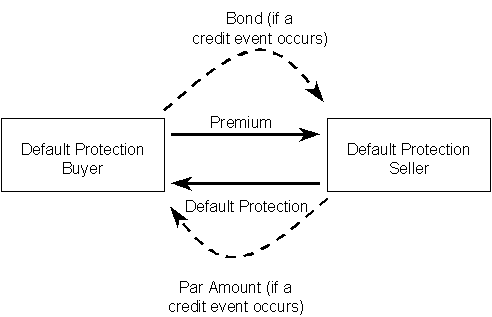
\includegraphics{fig2.png}}
		\caption{Credit Default Swap}
		\label{f2_a}
\end{figure}
 
\hspace{1cm} For example, suppose a company wants to raise money by issuing bonds that pays 5\% interest over 10 years. At maturity the bond principal has to be paid off by the company.
The bond buyer has taken risk by assuming that before maturity they will receive 5\% interest each year and at maturity they will receive their principal. Since their is always a chance that bond issuer will default, the bond purchaser may choose to allocate some part of interest towards the purchase of CDS swap. Then the CDS seller will pay the principal amount if the bond issuer defaults. Thus, CDS is used to hedge a position in corporate bond and due to this effect the corporate bond becomes risk free bond. Usually the payoff from a CDS will be $L(1-R)$, where L is notional principal and R is the Recovery rate.
\begin{itemize}
	\item \textbf{Valuation of Credit Default swaps}\label{itm:xyz}
	\medskip
	
	CDS spreads can be calculated using default probability estimates. The default probabilities used for this purpose should be risk-neutral default probabilities not the real world probabilities. If we assume that the probability of reference entity defaulting in a year conditional to no earlier default is X\% then the probability of survival is (100-X)\% for the first year. For the second year the probability of default conditional to no earlier default is X(100-X)\% while survival probability is (100-X(100-X))\%. Here we are assuming that defaults always happen halfway through the year and payments are made once at the end of each year. \medskip
	
	\hspace{1 cm}Expected payment of each year is given by the probability of survival of that year multiplied by payment rate s per year. Present value of expected payment of each year is expected payment multiplied by $e^{-rt}$ where r is the risk free rate and t is the value of that particular year. Adding present values of expected payment of each year will give total present value of expected payment.Expected accrual payment is the sum of adding present value of accrual payments of each year which is given by multiplying $e^{-rt}$ to accrual payments of each year where accrual payments are equal to default probability multiplied by $0.5s$ \medskip
	
	\hspace{1 cm}Expected payoff of each year is given by default probability multiplied by (1-R) where R is recovery rate. Present value of expected payoff of each year is expected payoff multiplied by $e^{-rt}$. Adding present values of expected payoff of each year will give total present value of expected payoff.\medskip
	
	\hspace{1 cm} Since, the present value of expected payoff is equal to the sum of present value of expected payment and present value of expected accrual payment(in case of default we have to pay halfway through the year). Using this relation we can easily find the value of X\% or s\%.\medskip
	    
	  \item \textbf{Marking to market of CDS} 
	  \medskip
	  
	  Suppose we have negotiated a CDS for a spread of 150 basis points then our s will become 0.015. Then, we calculate s from the method shown \hyperref[itm:xyz]{above}. If the calculated value$(s_1)$ is greater than s then the value of swap to the seller will be $(s_1-s)*principal$ and if value of $(s_1)$ is smaller then the value of swap to the buyer will become $(s-s_1)*principal $ . 
	 
	 \item \textbf{Binary Credit Default Swaps} 
	  \medskip
	  
	   In these kind of swaps payoff should be a fixed amount. It should not vary from time to time. In this case default probabilities are proportional to 1/(1-R) but payoffs are independent of R.  
	  \end{itemize}
	  
	   
	   \subsection{CDS forwards and options} 
	  \medskip
	  
	   Forward CDS comes into life at some future start date, provided that no default event occurs up till its start date. Otherwise, the contract to enter into the swap is nullified and no exchange of payments is made. If no default has occurred by the future start date, a credit default swap is entered into at that specified date. In other words, a forward CDS is a contract that obligates the holder to buy or sell a CDS on a particular reference entity for a preset spread (the forward CDS spread) at a future time. For example, a forward CDS might provides for the purchase of four year protection on firm A starting in one year for 250 basis points. If firm A defaults within the forward's life (i.e., one year), the swap dies out.\medskip
	   
	   \hspace{1 cm} A CDS option gives its holder the right, but not the obligation, to buy (call) or sell (put) protection on a specified reference entity for a specified future time period for a certain spread. The option is nullified if the reference entity defaults during the life of the option.Options on CD index swaps give investors the right to buy or sell risks at the strike spread. A \textbf{Payer Swaption} is an option that gives the holder the right to be the premium payer (protection buyer), while a \textbf{Receiver Swaption} is an option in which holder has the right to be the premium receiver (protection seller). A payer swaption is often referred to as a put (right to sell risk), a receiver swaption as a call (right to buy risk). For example, if the investor negotiates to buy protection on a credit starting on 1 year for s basis points, this is a call option and is exercised if the CDS spread  is more than s basis points. 
	   
	   \subsection{Total Return Swap}
	   \medskip
	   
	   It is a Type of credit derivative used to exchange the total return on a bond or any portfolio of assets for LIBOR plus a spread. The total return includes coupon, interest, gain or loss on the asset over the life of the swap..   
\begin{figure}[H]
		\centering
		\resizebox{0.6\linewidth}{!}{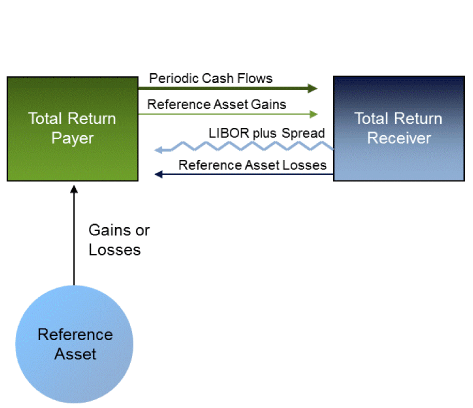
\includegraphics{fig3.png}}
		\caption{Total Return Swap}
		\label{f3_a}
\end{figure}
\pagebreak
 \hspace{1cm}Suppose, the receiver wants to buy a particular bond. Then, he approaches the payer and agrees to the swap. The payer then invest in the bond and retain it's ownership for the entire life of bond without giving it to the receiver to reduce risk. Actually, the receiver pays LIBOR and spread to the payer 
and the payer in return provides total return on the bond to the receiver as shown in \hyperref[f3_a]{Figure 3}. For example, suppose the two parties agrees to the terms of swap and buyer pays \$10 million for the bond. If the bond price increases by 10\% the buyer will pay \$1 to the receiver along with coupons and in return will get LIBOR plus spread. If the bond price decreases by 10\% then the receiver will pay 1\$ to the buyer along with LIBOR and spread.

 \subsection{Basket Credit Default Swap}
  \medskip
	   
In basket credit default swaps there are a number of reference entities. An \textbf{add up basket CDS} provides a payoff when any of the reference entities default while an \textbf{nth-to default CDS} provides payoff when the nth default occurs. After default, settlement takes place and swap then terminates without any further payment.

 \subsection{Collateralized Debt Obligations}
	   \medskip  
	   
Collateralized debt obligations (CDOs) are a type of structured asset-backed security with multiple ``tranches'' that are issued by special purpose entities and collateralized by debt obligations including bonds and loans. Each tranche offers a varying degree of risk and return so as to meet investor demand. CDOs' value and payments are derived from a portfolio of fixed-income underlying assets. CDO securities are split into different risk classes, or tranches, whereby ``senior" tranches are considered the safest securities and provides less yield while the highly risky tranches provide more yield and are referred to as \textbf{equity tranche}.  
\begin{figure}[H]
		\centering
		\resizebox{0.6\linewidth}{!}{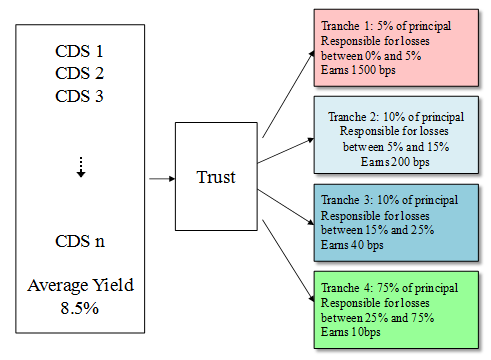
\includegraphics{fig4.png}}
		\caption{Collateralized Debt Obligation}
		\label{f4_a}
\end{figure} 

\hspace{1cm}From \hyperref[f4_a]{Figure 4} it is quite clear that tranche 1 has the maximum return and more risky while the tranche 4 has less return and less risky. For Example, suppose the whole amount is \$10000. Initially \$1500,\$200,\$40 and \$10 are provided to each of the tranches 1,2,3,4 respectively. 
Now if we loss \$1\% of the total bond then our total amount will become \$9000 in which tranche 2,3,4 will have same previous gain but tranche 1 principal reduces to \$400 instead of \$500 and hence without affecting any of the tranches, tranche 1 losses money. Thus, the tranche 1 have more risk and is given a low rating while the tranche 4 which is least probable to loose money has been given a high rating. \medskip


\hspace{1cm} If the creator of CDO sells a portfolio of credit default swaps to the third parties then it is called \textbf{Synthetic CDO}. Here, the first tranche might be responsible for the payoffs on the credit default swap until they have reached 5\% of the total notional principal; the second tranche might be responsible for payoff between 5\% and 15\% of total notional principal; and so on.
  \begin{itemize}
  	\item\textbf{Valuation of CDO using Gaussian Copula model of time of default}\medskip
  	
  	The valuation of a tranche of CDO is dependent on default correlation. If the correlation is low the junior equity tranche is very risky and the senior tranches are very safe. As the default correlation increases the junior tranches become less risky and senior tranches become more risky. We know that  
\begin{center}
	$ Q(T|M)$ = $N \left(\frac{N^{-1}[Q(T)]-\sqrt{\rho}M}{\sqrt{(1-\rho)}}\right)  $
\end{center}
where $ Q(T|M) $ is the probability of default by time T conditional on the value of factor, M. If we denote probability of k defaults by time T conditional on M as $P(k,T|M)$ then by properties of binomial distribution we get 
\begin{center}
	$P(k,T|M)$ = $\frac{N!}{(N-K)!k!} Q(T|M)^{k}[1- Q(T|M)]^{N-k}$
\end{center}
The probability that the nth default will happen between time $T_1$ and $T_2$ conditional on M is $P(n,T_2|M)$ - $P(n,T_1|M)$. To value the tranche of a CDO, we calculate expected payoffs and payments on the tranche conditional on M and the integrate over M.
  \end{itemize}
  
 \subsection{Convertible Bonds}
 \medskip
 
 It is a type of bond that the holder can convert into a specified number of shares of common stock in the issuing company or cash of equal value. It is a hybrid security with debt and equity like features. Convertible bonds are most often issued by companies with a low credit rating and high growth potential. Convertible bonds are bonds issued by a company where the holder has the option to exchange the bonds for the companies stock at certain time in future. The holder always has the right to convert the bond once it has been called. Sometimes holders call option is conditional on the price of company's stock being above a certain level. Thus, convertible bonds allow issuers to issue debt at a lower cost. Typically, a convertible bond at issue yields 1\% to 3\% less than straight bonds.
\end{document}
